\documentclass[main.tex]{subfiles}

\begin{document}

\section{Introduzione}\label{sec:introduzione}

\hspace*{0.25in}L'idea del progetto nasce dalla volontà di approfondire il modo di creazione e di manipolazione delle immagini, introdotto durante il corso. L'idea iniziale era di creare un Ray Tracer real-time da testare su un videogioco semplice, come Doom, ma ci siamo subito accorti che sarebbe stata un'impresa troppo grande. Nulla vieta che il progetto potrebbe essere esteso in futuro con più calma. \\
Ciò che abbiamo fatto, invece, è stato creare un Ray Tracer di immagini statiche ad alta definizione utilizzando le tecniche di parallelizzazione di CUDA. Abbiamo analizzato il le prestazioni e cercato di ottimizzarle, ottenendo discreti risultati su alcuni aspetti.

\subsection{Ray Tracing}

\hspace*{0.25in}Non conoscendo le basi dietro il funzionamento dei Ray Tracer, abbiamo studiato con molto interesse il libro \textit{Ray Tracing in One Weekend} \cite{Shirley2023RTW1}. \\
La parola Ray Tracing cela, difatti, un vasto insieme di tecniche che sfruttano la geometria ottica per comprendere ed emulare il percorso dei raggi della luce e le loro interazioni con le superfici. Queste tecniche vengono utilizzate sia nella modellazione di sistemi ottici, come le lenti delle fotocamere, sia nella Computer Grafica, per simulare la luce e la riflessione in modo più realistico. \\
A differenza di altri metodi di rendering, il ray tracing simula il percorso della luce nel modo più fedele possibile. Il processo inizia con la generazione di raggi di luce virtuali che partono dalla sorgente luminosa e vengono tracciati attraverso la scena virtuale. Ogni raggio può interagire con gli oggetti incontrati nel suo percorso, dando luogo a fenomeni come riflessione, rifrazione, ombre e illuminazione globale.\\ 
Le fasi principali del Ray Tracing includono:
\begin{enumerate}
    \item Lancio dei Raggi (Ray Casting): vengono generati raggi dalla sorgente luminosa attraverso ogni pixel dell'immagine;
    
    \item Intersezione dei Raggi: i raggi vengono tracciati attraverso la scena, e quando incontrano un oggetto, viene calcolato il punto di intersezione;

    \item Calcolo della Luce: in base alle caratteristiche dei materiali degli oggetti e alle proprietà della luce, vengono calcolati i valori di colore per ogni pixel.

    \item Rendering Finale: l'immagine finale viene composta con tutti i calcoli effettuati per ogni pixel, creando un'immagine realistica e dettagliata.
\end{enumerate} 
Il ray tracing è noto per produrre risultati visivi eccezionali, ma richiede notevoli risorse computazionali e può essere un processo intensivo in termini di tempo. Tuttavia, con l'avanzare della tecnologia hardware, l'utilizzo del ray tracing sta diventando sempre più diffuso nei settori dell'intrattenimento digitale, offrendo esperienze visive sempre più immersive e realistiche.


\subsection{CUDA (Compute Unified Device Architecture)}
\hspace*{0.25in}CUDA è una piattaforma di calcolo parallelo per l'utilizzo delle GPU NVIDIA, progettate apposta per gestire una grande quantità di operazioni simultanee. Poiché il Ray Tracing coinvolge una grande quantità di calcoli parallelizzabili, la loro architettura è particolarmente adatta ad affrontare questa mole di lavoro in modo efficiente. \\
Come già citato, è noto lo svantaggio in termini di performance degli algoritmi di Ray Tracing rispetto ad altri come lo Scanline Rendering \cite{ScanlineAlgo} che utilizza la coerenza dei dati per gestire la computazione tra i pixel. La scelta di trattare ogni raggio in modo separato fa ricominciare tutto il procedimento ad ogni nuovo pixel e se da un lato questo offre il vantaggio di migliorare la qualità dell'immagine, dall'altro genera un notevole impiego di risorse.\\ 
Il lancio dei raggi, però, può essere eseguito in modo parallelo tramite i CUDA threads assegnando la computazione di un pixel ad ogni thread. Questo approccio consente di gestire scenari più complessi e di aumentare la risoluzione delle immagini senza subire un degrado significativo delle prestazioni. \\

\begin{figure}[h]
    \centering
    \fbox{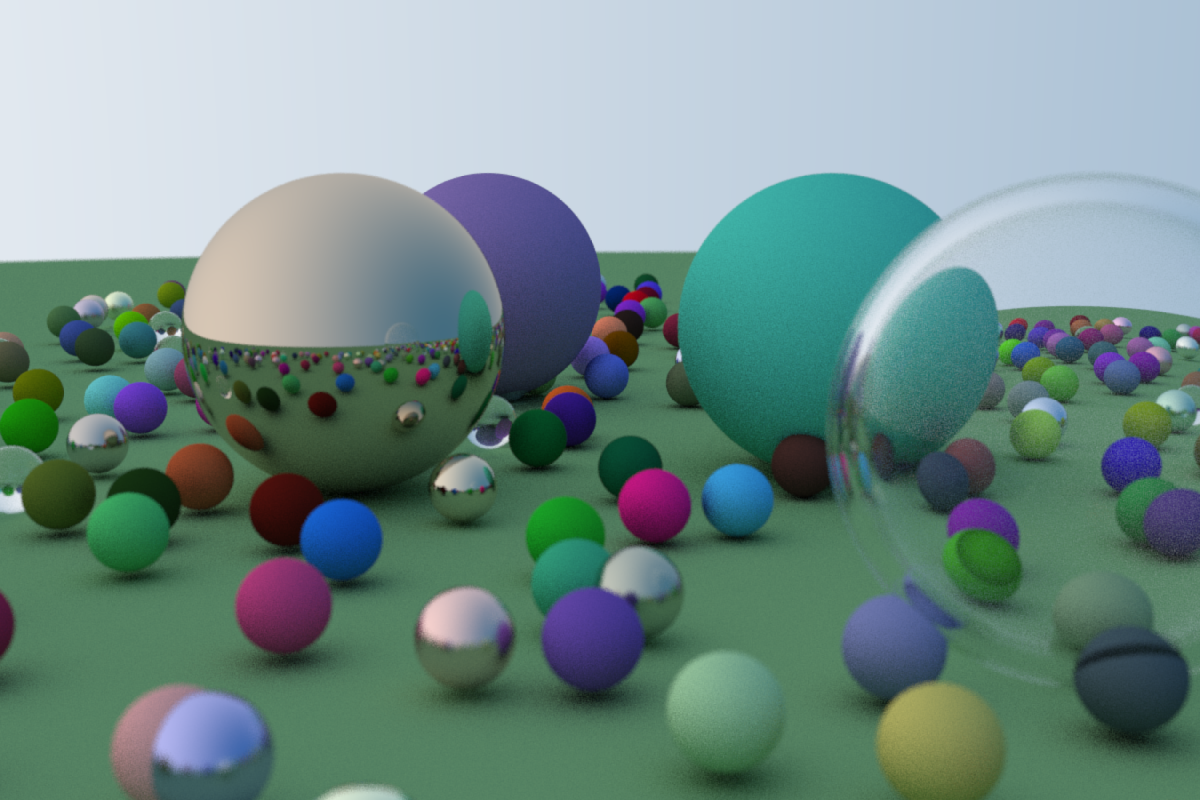
\includegraphics[width=0.8\linewidth]{figures/giorno.png}}
    \caption{Immagine generata con Ray Tracing}\vspace{-14pt}\rule{0.55\linewidth}{0.4pt}
\end{figure}

\end{document}